\documentclass{standalone}
\usepackage{tikz}
%------------tikz Setup------------

\tikzstyle{ball} = [circle,shading=ball, ball color=black,
    minimum size=1mm,inner sep=1.3pt]
\tikzstyle{miniball} = [circle,shading=ball, ball color=black,
    minimum size=1mm,inner sep=0.5pt]
\tikzstyle{mminiball} = [circle,shading=ball, ball color=black,
    minimum size=0.6mm,inner sep=0.1pt]
\usetikzlibrary{arrows.meta}
\usetikzlibrary{angles, quotes}
\tikzset{>={Latex[length=2mm,width=1.5mm]}}
\tikzset{->-/.style={decoration={markings, mark=at position #1 with
  {\arrow{>}}},postaction={decorate}}}
\usetikzlibrary{decorations.pathmorphing}
\usetikzlibrary{decorations.pathreplacing}
\usetikzlibrary{arrows.meta,calc}
\usetikzlibrary{bending}
\usetikzlibrary{decorations.markings,shapes.geometric}
\tikzset{->-/.style={decoration={markings, mark=at position #1 with
  {\arrow{>}}},postaction={decorate}}}
\tikzset{-|-/.style={decoration={markings, mark=at position #1 with
  {\arrow{stealth}}},postaction={decorate}}}
\tikzset{movearrow/.style 2 args ={
        decoration={markings,
    mark= at position {#1} with {\arrow{#2}} ,
        },
        postaction={decorate}
    }
}


\begin{document}
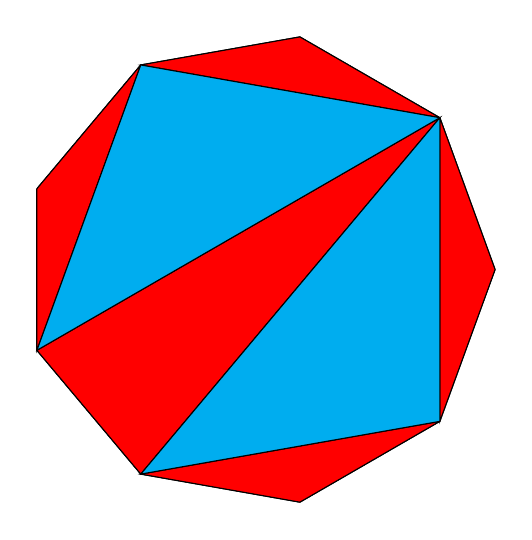
\begin{tikzpicture}
\begin{scope}[scale=3]
    \def\deg{40}    %interior angle
    %original pentagon
    \foreach [evaluate={
        \t=int(\x*\deg);
        }]\x in {1,2,...,9}
    {\node (\x) at (\t:1) {};}
    \foreach \from/\to in {1/2, 2/3, 3/4, 4/5, 5/6, 6/7, 7/8, 8/9, 9/1}
    {\draw (\from.center) -- (\to.center);}
    \draw[fill=red] (1.center) -- (2.center) -- (3.center) -- (1.center);
    \draw[fill=red] (3.center) -- (4.center) -- (5.center) -- (3.center);
    \draw[fill=red] (1.center) -- (9.center) -- (8.center) -- (1.center);
    \draw[fill=red] (8.center) -- (7.center) -- (6.center) -- (8.center);
    \draw[fill=red] (6.center) -- (5.center) -- (1.center) -- (6.center);
    \draw[fill=cyan] (1.center) -- (3.center) -- (5.center) -- (1.center);
    \draw[fill=cyan] (1.center) -- (8.center) -- (6.center) -- (1.center);
\end{scope}
\end{tikzpicture}
\end{document}